%- block legend
Uma \textit{string} de abre e fecha parênteses está \textit{bem balanceada} se:
ou é $($ seguido de uma \textit{string} bem balanceada seguida de $)$;
ou é a concatenação de duas \textit{strings} bem balanceadas;
ou é vazia (formalmente, é uma \textit{string} gerada pela gramática $S \rightarrow (S) | SS | \varepsilon$).

É dada uma \textit{string} inicial $s$ com $N$ parênteses. Processe $Q$ operações, onde cada operação pode ser:
\begin{itemize}
    \item $1$ $l$ $r$: inverta todos os parênteses no intervalo
    $[l..r]$; isto é,
    para todo $l \leq i \leq r$, troque $s[i]$ pelo inverso de $s[i]$. O
    \textit{inverso} de $)$ é $($, enquanto o inverso de $($ é $)$;
    \item $2$ $l$ $r$: determine se a \textit{substring} $s[l..r]$ está bem balanceada.
\end{itemize}

%- endblock

%- block input
A primeira linha contém dois inteiros $N$ e $Q$
($1 \leq N, Q \leq \VAR{vars.N.max | sci}$), o tamanho da \textit{string} e o
número de operações.
A segunda linha contém a \textit{string} inicial com $N$ parênteses.
As próximas $Q$ linhas descrevem uma operação cada, na forma
$t$ $l$ $r$ onde $t=1$ ou $t=2$, e $1 \leq l \leq r \leq N$.

%- endblock

%- block output
Para cada operação com $t=2$, imprima uma linha com \texttt{sim} se a \textit{substring}
$s[l..r]$ está bem balanceada, ou \texttt{nao} caso contrário.
%- endblock

%- block notes
Considere o primeiro exemplo dado.
Na primeira operação, a resposta é \texttt{sim} porque
$s[6..9] = $\texttt{()()} está bem balanceada. Na segunda operação, a resposta é
\texttt{nao} porque $s[1..10]$ = \texttt{()())()())} não está bem balanceada.

Após a terceira operação (inverte $s[4..6]$), a \textit{string} se torna
\texttt{()((())())}. A resposta da quarta operação é \texttt{sim} porque agora
$s[1..10]$= \texttt{()((())())} está bem balanceada.

%- endblock

%- block editorial
É bastante conhecido o algoritmo de verificação que usa uma pilha como estrutura auxiliar ou,
neste caso em que há apenas um tipo de parênteses, um contador com o tamanho da
pilha: incremente o contador ao encontrar $($ e decremente o contador ao
encontrar $)$. Para ser bem balanceada, o contador deve terminar em 0 (zero) e
nunca pode ter assumido algum valor negativo (menor que zero) durante o
algoritmo.

Esta ideia é equivalente a considerar $($ como +1 e $)$ como -1, e, dado um
intervalo, verificar se a
soma de todos os seus valores é 0 e também se não existe nenhum
prefixo do intervalo cuja soma é
negativa. O gráfico abaixo exemplifica a soma dos prefixos para
\texttt{()(())}, que é bem balanceada; note que termina em 0 e nunca fica abaixo
de 0 no gráfico.

\begin{center}
    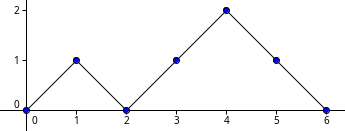
\includegraphics[scale=1.9]{graficocerto.png}
\end{center}

Apenas utilizar esse algoritmo a cada operação do
tipo 2 faria a solução ter uma complexidade de $O(Q \times N)$, que é muito
lento para os limites deste problema. Precisamos de uma estrutura de dados
auxiliar que, dado um intervalo $[l..r]$, permita determinar a soma dos valores
no intervalo, e também o valor da menor soma de um prefixo do intervalo (ambos
devem ser iguais a 0 para a \textit{substring} ser balanceada). Com uma
\textbf{Árvore de Segmentos}, podemos determinar ambos os valores em $O(\lg N)$,
    o que é rápido o bastante.

Nos resta saber como atualizar a árvore a cada operação do
tipo 1. Vamos notar o que acontece com as somas dos prefixos do intervalo quando
ele é invertido; os gráficos abaixo exemplificam a soma dos prefixos para
\texttt{(()))((} e seu inverso \texttt{))((())}, que não são bem balanceados:

\begin{center}
    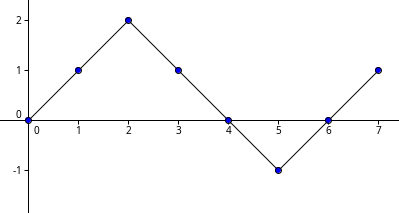
\includegraphics[scale=1.6]{grafico1.png}$ $
    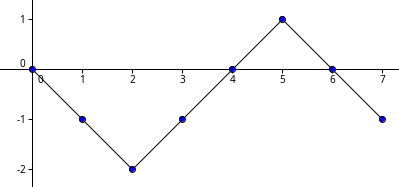
\includegraphics[scale=1.6]{grafico2.png}
\end{center}

Note que o gráfico apenas se ``espelha verticalmente'', de forma que: a soma do intervalo tem seu sinal invertido; o novo valor mínimo do
intervalo passa a ser o antigo valor máximo do intervalo, com sinal invertido; e
o novo valor máximo do intervalo passa a ser o o antigo valor mínimo, também com
sinal invertido. Assim, é possível processar cada operação em $O(\lg N)$ com a técnica de
\textbf{Lazy Propagation}, mantendo em
cada nodo da árvore a soma, o menor valor e o maior valor dos prefixos do
segmento, e os atualizando conforme as propriedades de ``espelhamento'' citadas.

Uma referência para a Árvore de Segmentos e Lazy Propagation é
\url{https://cp-algorithms.com/data_structures/segment_tree.html}.

Complexidade total: $O(N + Q\lg N)$
%- endblock
